\documentclass[a4paper, fontsize=11pt]{scrartcl} % A4 paper and 11pt font 
\usepackage[a4paper,left=3cm,right=2cm,top=2.5cm,bottom=2.5cm]{geometry}

\usepackage[T1]{fontenc} % Use 8-bit encoding that has 256 glyphs
\usepackage{fourier} % Use the Adobe Utopia font for the document - comment this line to return to the LaTeX default
\usepackage[spanish]{babel} % Spanish language/hyphenation
\selectlanguage{spanish}
\usepackage[utf8]{inputenc}
\usepackage{amsmath,amsfonts,amsthm} % Math packages
\usepackage{graphicx} % The graphicx package
\usepackage{placeins}
\usepackage{caption}
\usepackage{subcaption}

\usepackage{cite} % para contraer referencias
\usepackage{hyperref}

\usepackage{listings} % Insert Scripts
\usepackage{color} %red, green, blue, yellow, cyan, magenta, black, white
\definecolor{mygreen}{RGB}{28,172,0} % color values Red, Green, Blue
\definecolor{mylilas}{RGB}{170,55,241}

\lstset{language=Matlab,%
	%basicstyle=\color{red},
	breaklines=true,%
	morekeywords={matlab2tikz},
	keywordstyle=\color{blue},%
	morekeywords=[2]{1}, keywordstyle=[2]{\color{black}},
	identifierstyle=\color{black},%
	stringstyle=\color{mylilas},
	commentstyle=\color{mygreen},%
	showstringspaces=false,%without this there will be a symbol in the places where there is a space
	numbers=left,%
	numberstyle={\tiny \color{black}},% size of the numbers
	numbersep=9pt, % this defines how far the numbers are from the text
	emph=[1]{for,end,break},emphstyle=[1]\color{red}, %some words to emphasise
	%emph=[2]{word1,word2}, emphstyle=[2]{style},    
}

\usepackage{sectsty} % Allows customizing section commands
%\allsectionsfont{\centering \normalfont\scshape} % Make all sections centered, the default font and small caps

\usepackage{fancyhdr} % Custom headers and footers
\pagestyle{fancyplain} % Makes all pages in the document conform to the custom headers and footers
\fancyhead{} % No page header - if you want one, create it in the same way as the footers below
\fancyfoot[L]{} % Empty left footer
\fancyfoot[C]{} % Empty center footer
\fancyfoot[R]{\thepage} % Page numbering for right footer
\renewcommand{\headrulewidth}{0pt} % Remove header underlines
\renewcommand{\footrulewidth}{0pt} % Remove footer underlines
\setlength{\headheight}{13.6pt} % Customize the height of the header

\numberwithin{equation}{section} % Number equations within sections (i.e. 1.1, 1.2, 2.1, 2.2 instead of 1, 2, 3, 4)
\numberwithin{figure}{section} % Number figures within sections (i.e. 1.1, 1.2, 2.1, 2.2 instead of 1, 2, 3, 4)
\numberwithin{table}{section} % Number tables within sections (i.e. 1.1, 1.2, 2.1, 2.2 instead of 1, 2, 3, 4)

%\setlength\parindent{0pt} % Removes all indentation from paragraphs - comment this line for an assignment with lots of text

\newenvironment{myalign}{\par\nobreak\large\noindent\align}{\endalign} %Altering fontsize in equations globally

%----------------------------------------------------------------------------------------
%	TITLE SECTION
%----------------------------------------------------------------------------------------

\newcommand{\horrule}[1]{\rule{\linewidth}{#1}} % Create horizontal rule command with 1 argument of height

\title{	
	\normalfont \normalsize 
	\textsc{Master en Automática y Robótica - UPM} \\ [25pt] % Your university, school and/or department name(s)
	\horrule{0.5pt} \\[0.4cm] % Thin top horizontal rule
	\huge Práctica de Telerrobótica y Teleoperación \\ % The assignment title
	\horrule{2pt} \\[0.5cm] % Thick bottom horizontal rule
}

\author{Jorge Camarero Vera - 07052} % Your name

\date{\normalsize\today} % Today's date or a custom date

\begin{document}
	\maketitle
	
	\section{Explicación de la tarea}
	
	Sea un sistema de telemanipulación maestro/esclavo con la siguiente dinámica:
	%
	\begin{myalign}
		\begin{split}
			M_m\ddot{x}_m(t) &= -K_ff_{md}(t) - B_m\dot{x}_m(t) - K_hx_m(t)\\
			M_s\ddot{x}_s(t) &= f_s(t) - B_s\dot{x}_s(t)
		\end{split}
	\label{Model Equations}
	\end{myalign}
	%
	donde:
	\begin{itemize}
		\item $M_{m,s} = 1$, $B_{m,s}=20$, masa y fricción, respectivamente, de maestro y esclavo.
		\item $K_h=K_f = 100$, constantes de elasticidad del operador.
	\end{itemize}
	
	Se pide construir los modelos bilaterales en Matlab/Simulink \textbf{posición-posición} y \textbf{fuerza-posición}. Comprobar su funcionamiento con movimiento libre, entorno elástico y entorno viscoso.

	%\begin{figure}[h!]
	%	\centering
	%	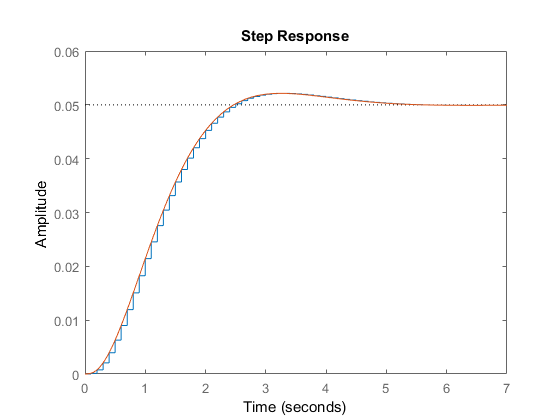
\includegraphics[width=1.0\linewidth]{images/ComparedOutput.png}
	%	\caption{Salida discreta y continua del sistema controlado ante entrada escalón unitario.}
	%	\label{Compared Output}
	%\end{figure}
	%\FloatBarrier
	
	\subsection{Creación de los modelos}\label{Models Creation}
	
	Para la realización de los modelos Posición-Posición y Fuerza-Posición ha sido tomada como referencia los diagramas de control de las Figuras \ref{Position-Position Control Scheme} y \ref{Force-Position Control Scheme} \cite{Bilateral}.\\
	
	\begin{figure}[h]
		\centering
		\begin{subfigure}[t]{.5\textwidth}
			\centering
			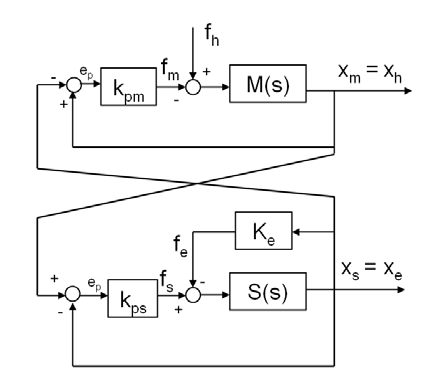
\includegraphics[width=1\linewidth]{images/Position-Position.PNG}
			\caption{Esquema de control Posición-Posición}
			\label{Position-Position Control Scheme}
		\end{subfigure}%
		\begin{subfigure}[t]{.5\textwidth}
			\centering
			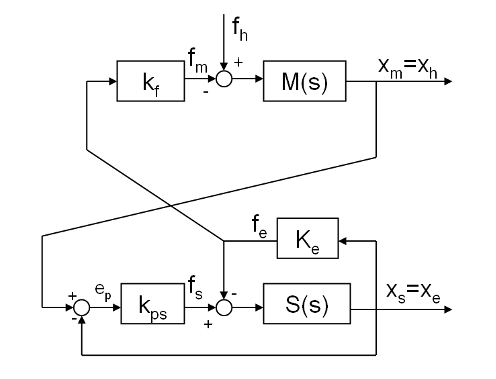
\includegraphics[width=1\linewidth]{images/Force-Position.PNG}
			\caption{Esquema de control Fuerza-Posición}
			\label{Force-Position Control Scheme}
		\end{subfigure}
		\caption{Esquemas de control Bilateral}
		\label{Control Schemes}
	\end{figure}
	%\FloatBarrier
	
	En la creación de los modelos bilaterales primero habrá que modelizar tanto el maestro como el esclavo a partir de sus ecuaciones, descritas en (\ref{Model Equations}). Para el maestro obtenemos el modelo de la Figura \ref{Master}, y para el esclavo el de la Figura \ref{Slave}. Pero para el Maestro del modelo Fuerza-Posición ha sido sacada la Kf para parecerse más al esquema de la Figura \ref{Force-Position Control Scheme}, quedando el modelo de la Figura \ref{Modified Master}.\\
	
	Además la entrada de fuerza del operario a cada sistema, Posición-Posición y Fuerza-Posición, se ha modelado como pulsos de valor máximo 1 con un periodo de 10 segundo y el pulso tiene una duración de 1 segundo, esto se hace para evitar que los sistemas no generen inestabilidades fácilmente.\\
	
	\begin{figure}[h]
		\centering
		\begin{subfigure}[t]{.5\textwidth}
			\centering
			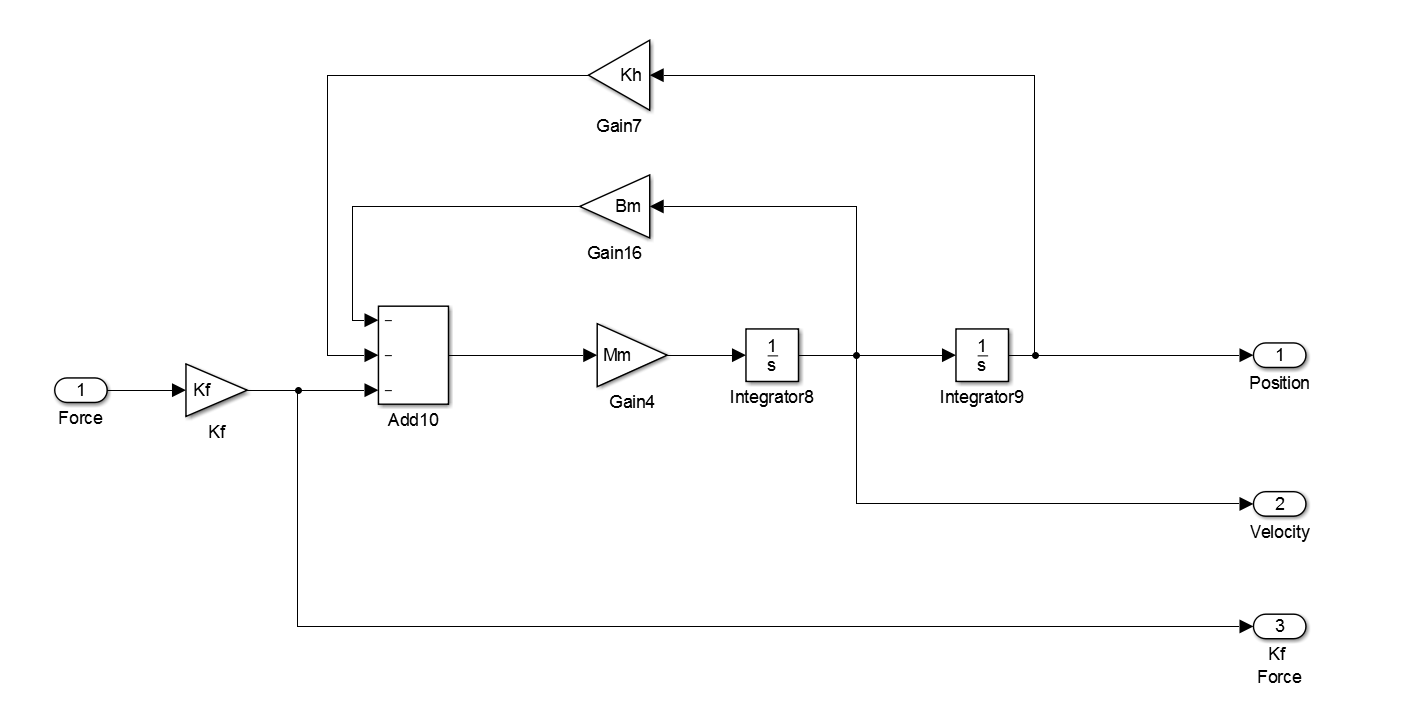
\includegraphics[width=1\linewidth]{images/Master.PNG}
			\caption{Modelo del Maestro}
			\label{Master}
		\end{subfigure}%
		\begin{subfigure}[t]{.5\textwidth}
			\centering
			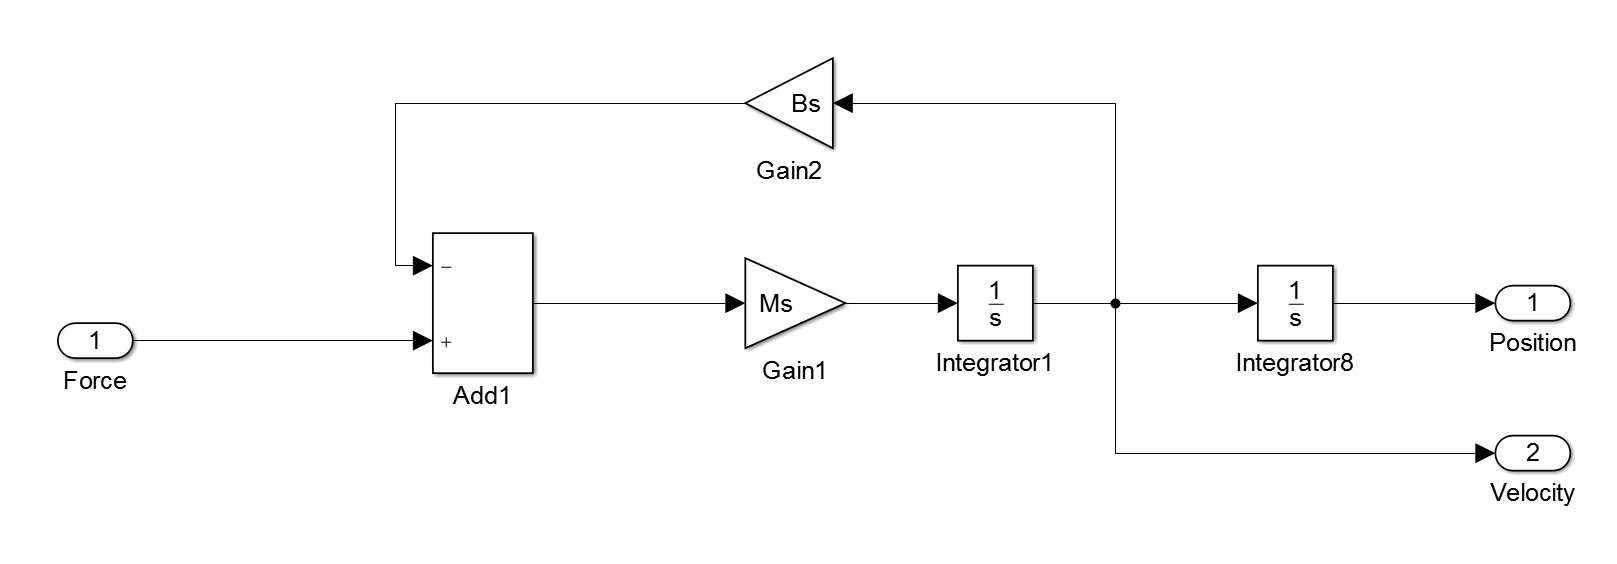
\includegraphics[width=1\linewidth]{images/Slave.PNG}
			\caption{Modelo del Esclavo}
			\label{Slave}
		\end{subfigure}
		\begin{subfigure}{\linewidth}
			\centering
			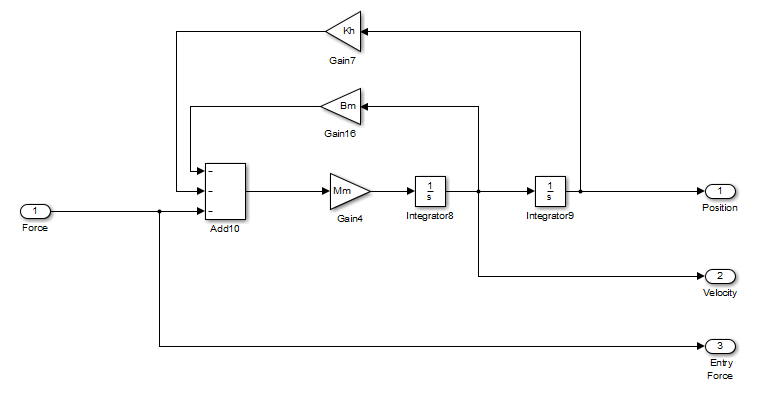
\includegraphics[width=0.5\linewidth]{images/Master_Mod.PNG}
			\caption{Modelo del Maestro modificado para el modelo Fuerza-Posición}
			\label{Modified Master}
		\end{subfigure}
		\caption{Modelos de Maestro y Esclavo para el modelo Posición-Posición y Fuerza-Posición}
		\label{Master_Slave}
	\end{figure}
	\FloatBarrier
	
	\pagebreak
		
	\subsubsection{Modelo Bilateral Posición-Posición}
	
	\begin{figure}[h!]
		\centering
		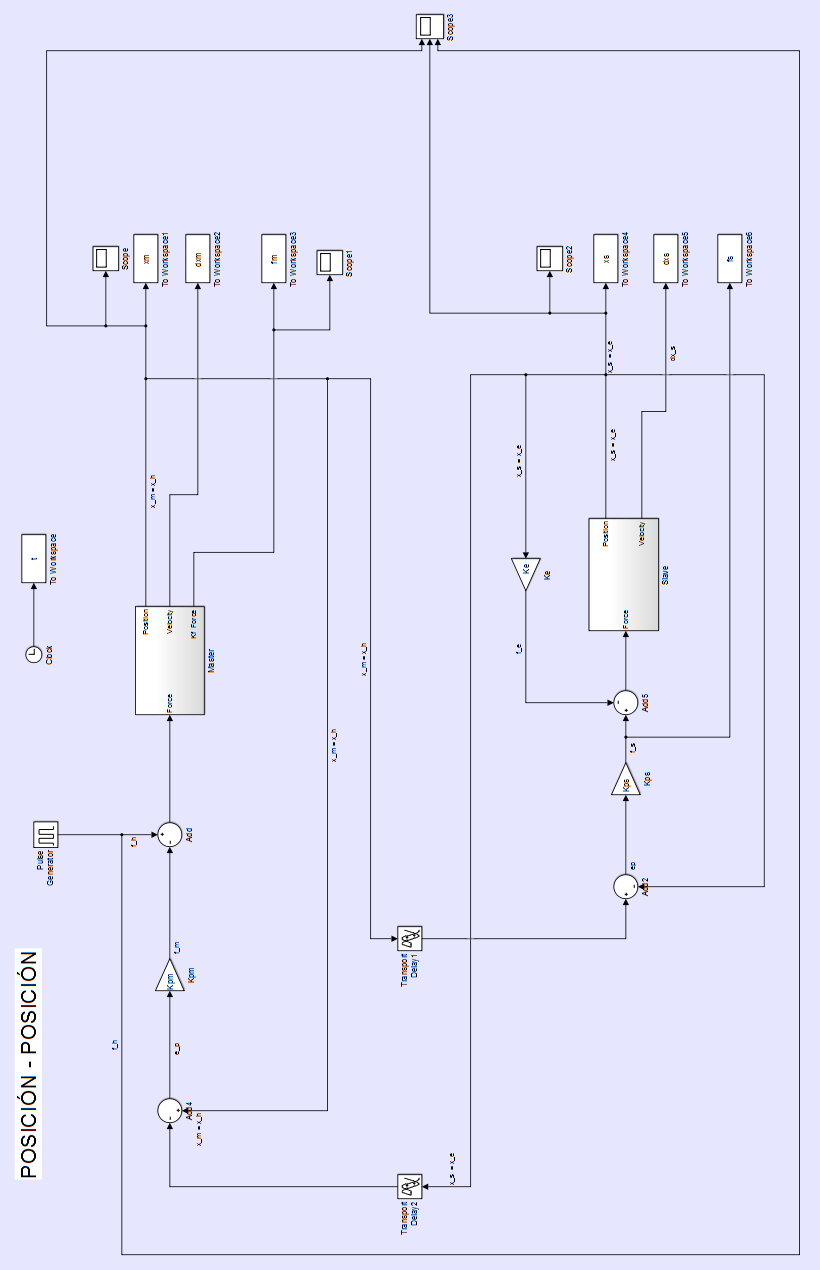
\includegraphics[height=1.42\linewidth]{images/Model_POS-POS.PNG}
		\caption{Modelo desarrollado de Posición-Posición}
		\label{Model Position-Position}
	\end{figure}
	\FloatBarrier
	
	Con lo anteriormente descrito, para modelizarlo fue creado en Simulink el sistema bilateral Posición-Posición, Figura \ref{Model Position-Position}. Se han tomado como predeterminados los siguientes valores:
	
	\begin{lstlisting}
	Bm = 20;
	Bs = 20;
	Kf = 100;
	Kh = 0;
	Kpm = 0.25;
	Kps = 100;
	Mm = 1;
	Ms = 1;
	Ke = 0;
	\end{lstlisting}
	\label{Predet1}
	%
	obteniéndose la Figura \ref{Predet Values}. Y observándose como la respuesta de posición del esclavo, $x_s$, va después del maestro, $x_m$, lo cuál cabe de esperar ya que es el maestro donde actúa el operador.\\
	
	\begin{figure}[h]
		\centering
		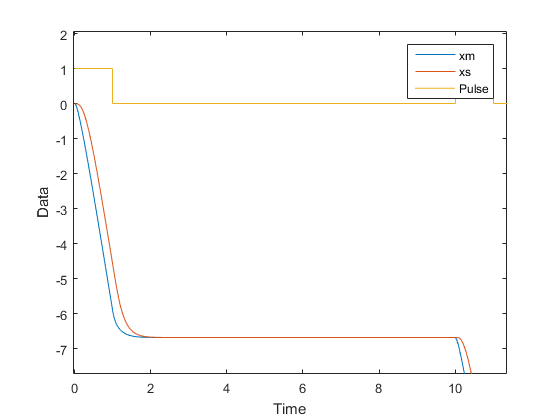
\includegraphics[width=0.5\linewidth]{images/Predet.PNG}
		\caption{Modelo con los valores predeterminados dados.}
		\label{Predet Values}
	\end{figure}
	\FloatBarrier

	Modificándose el valor de rozamiento en el maestro, $B_m$, se obtiene los resultados de la Figura \ref{Master_Friction}. Se observa que cuanto mayor es $B_m$ menor es la amplitud de respuesta del maestro y del esclavo ante un mismo pulso de fuerza. Estas respuestas son lógicas, ya que cuando con el medio o internamente el propio robot posee fricciones antes una misma fuerza el maestro se desplaza menos, al haber una fuerza que se le contrapone dependiente de la velocidad a la que se mueva el maestro.\\
	
	\begin{figure}[h!]
		\centering
		\begin{subfigure}[t]{.5\textwidth}
			\centering
			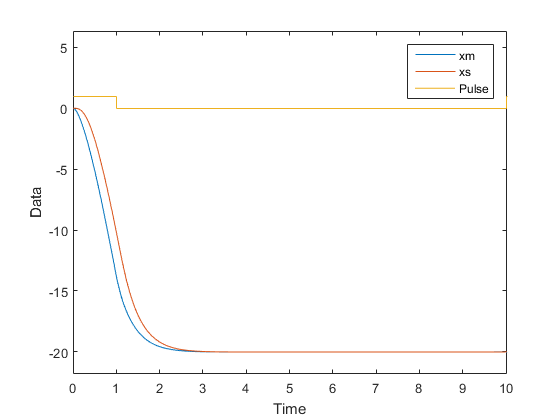
\includegraphics[width=1\linewidth]{images/Bm10.PNG}
			\caption{Con $B_m = 10$}
			\label{Bm10}
		\end{subfigure}%
		\begin{subfigure}[t]{.5\textwidth}
			\centering
			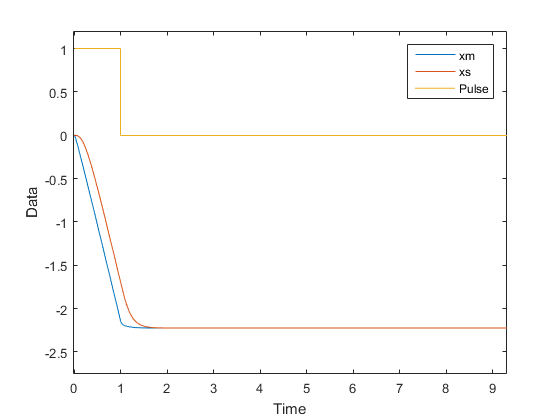
\includegraphics[width=1\linewidth]{images/Bm50.PNG}
			\caption{Con $B_m = 50$}
			\label{Bm50}
		\end{subfigure}
		\begin{subfigure}[t]{.5\textwidth}
			\centering
			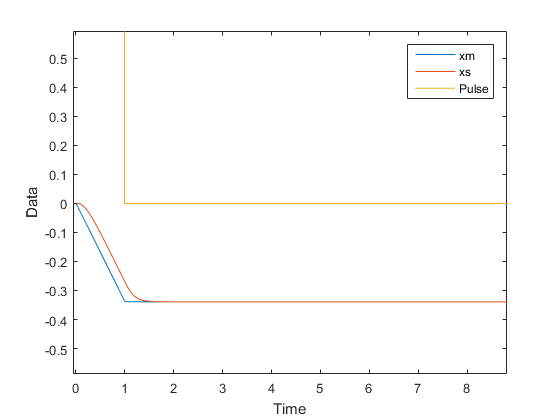
\includegraphics[width=1\linewidth]{images/Bm300.PNG}
			\caption{Con $B_m = 300$}
			\label{Bm300}
		\end{subfigure}
		\caption{Respuestas con distintos coeficientes de fricción en el Maestro}
		\label{Master_Friction}
	\end{figure}
	\FloatBarrier
	
	Manteniendo $B_m = 300$ modificamos el coeficiente $B_s$ de fricción del esclavo, obteniendo las respuestas respresentadas en las Figuras \ref{Slave_Friction}. Se observa que las amplitudes de las respuestas son parecidas, pero varía mucho las formas de la respuesta del sistema esclavo, esto es entendible ya que ante un mismo movimiento del maestro el esclavo actúa cada vez con menor movimiento, en la Figura \ref{Bs10}. Incluso se observa que el esclavo se desplaza más de lo debido creando una pequeña oscilación, como hay un bucle de realimentación al Maestro, este también muestra una aún más pequeña sobreoscilación. Al crecer la $B_s$ las diferencias de movimiento serán cada vez mayores, llegando a grandes discrepancias entre Maestro y Esclavo llevando al sistema a la inestabilidad.\\
	
	\begin{figure}[h!]
		\centering
		\begin{subfigure}[t]{.5\textwidth}
			\centering
			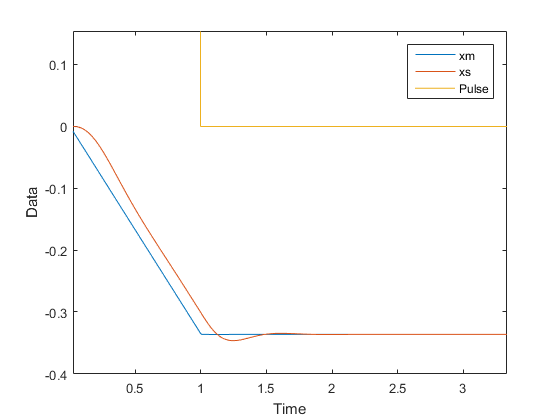
\includegraphics[width=1\linewidth]{images/Bs10.PNG}
			\caption{Con $B_s = 10$}
			\label{Bs10}
		\end{subfigure}%
		\begin{subfigure}[t]{.5\textwidth}
			\centering
			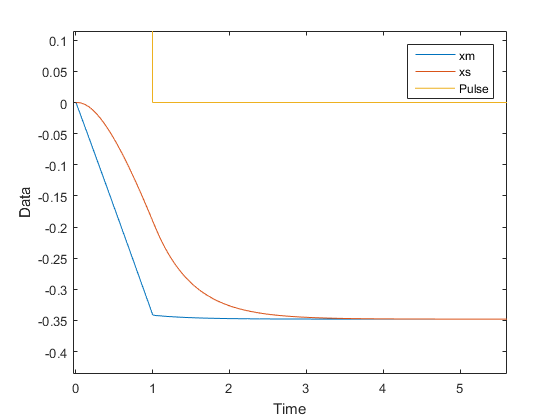
\includegraphics[width=1\linewidth]{images/Bs50.PNG}
			\caption{Con $B_s = 50$}
			\label{Bs30}
		\end{subfigure}
		\begin{subfigure}[t]{.5\textwidth}
			\centering
			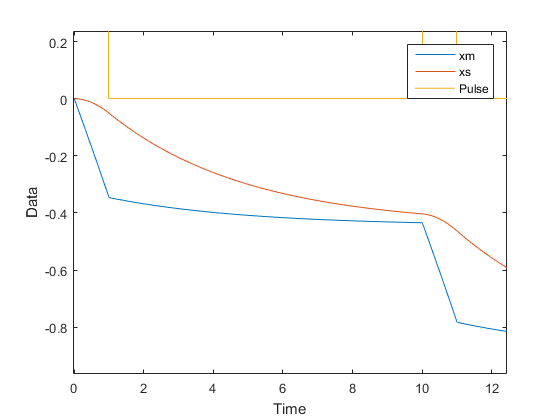
\includegraphics[width=1\linewidth]{images/Bs300.PNG}
			\caption{Con $B_s = 300$}
			\label{Bs300}
		\end{subfigure}
		\caption{Respuestas con distintos coeficientes de fricción en el Esclavo}
		\label{Slave_Friction}
	\end{figure}
	\FloatBarrier
	
	Todos estos casos en los que se han modificado los coeficientes de fricción se han realizado con un $K_e = 0$, por tanto el movimiento es libre, Ahora se pasará a estudiar los casos con $K_e > 0$, es decir el caso de estar en un entorno elástico y con fricción y/o viscosidad de $B_m = 300$ y $B_s = 100$. Entonces se obtienen las respuestas de la Figura \ref{Slave_Stifnes}. Al aumentar la coeficiente de elasticidad con el entorno la respuesta del esclavo ante el maestro va creciendo en error de posición con respecto a la posición del maestro, cuando se deja de aplicar fuerza, este fenómeno se entiende ya que cada vez cuesta más mover el esclavo debido a la existencia de ese \textquotedblleft muelle \textquotedblright. Además se ve que la respuesta del maestro no cambia al aumentar $K_e$, pero la diferencia que irá creciendo en la posición respecto al esclavo acabará con una gran inestabilidad en el sistema, a causa de la realimentación del control bilateral.\\
	
	\begin{figure}[h!]
		\centering
		\begin{subfigure}[t]{.5\textwidth}
			\centering
			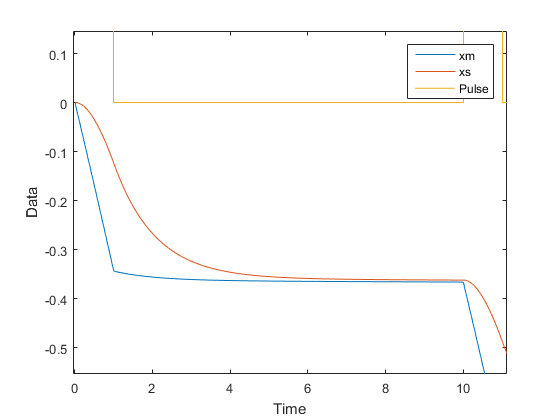
\includegraphics[width=1\linewidth]{images/Ke1.PNG}
			\caption{Con $K_e = 1$}
			\label{Ke1}
		\end{subfigure}%
		\begin{subfigure}[t]{.5\textwidth}
			\centering
			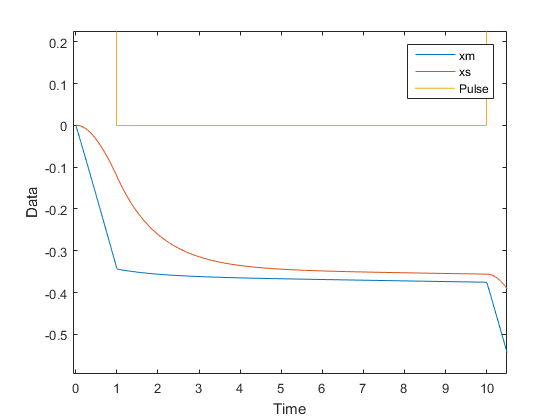
\includegraphics[width=1\linewidth]{images/Ke5.PNG}
			\caption{Con $K_e = 5$}
			\label{Ke5}
		\end{subfigure}
		\begin{subfigure}[t]{.5\textwidth}
			\centering
			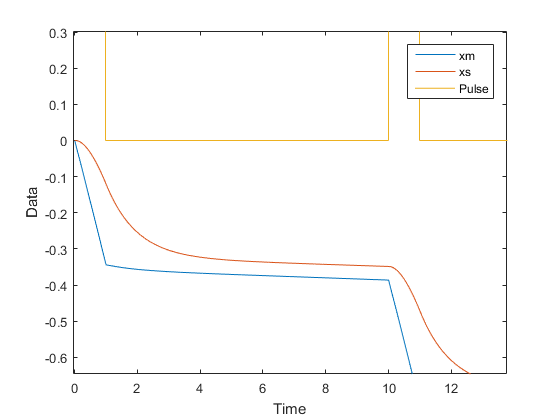
\includegraphics[width=1\linewidth]{images/Ke10.PNG}
			\caption{Con $K_e = 10$}
			\label{Ke10}
		\end{subfigure}
		\caption{Respuestas con distintos coeficientes de elasticidad, $K_e$, en el sistema esclavo}
		\label{Slave_Stifnes}
	\end{figure}
	\FloatBarrier
	
	\pagebreak
	
	\subsubsection{Modelo Bilateral Fuerza-Posición}
	
	\begin{figure}[h!]
		\centering
		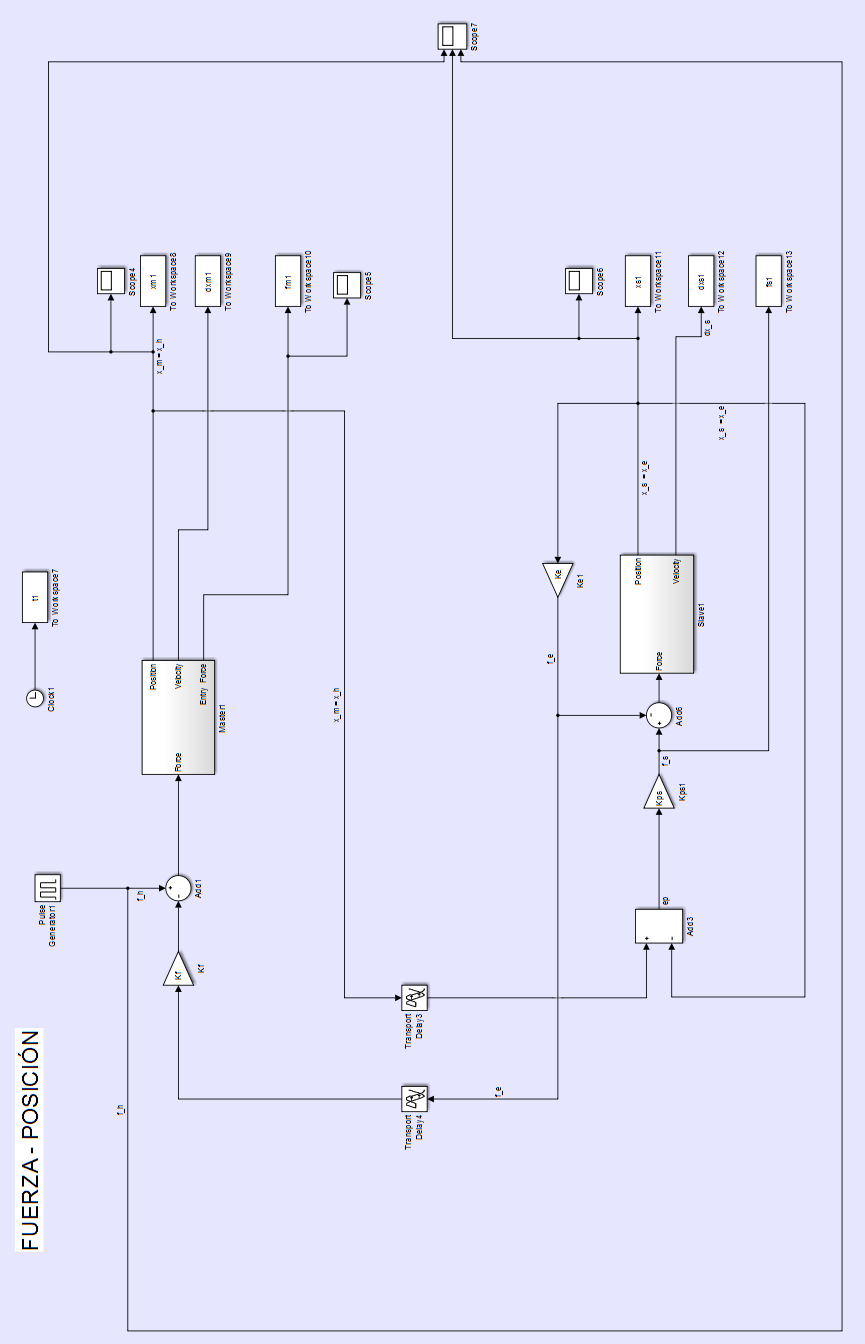
\includegraphics[height=1.42\linewidth]{images/Model_FOR-POS.PNG}
		\caption{Modelo desarrollado de Fuerza-Posición}
		\label{Model Force-Position}
	\end{figure}
	
	
	Con lo descrito en la Sección \ref{Models Creation}, para modelizarlo fue creado en Simulink el sistema bilateral Fuerza-Posición, Figura \ref{Model Force-Position}. Se han tomado como predeterminados los siguientes valores:
	
	\begin{lstlisting}
	Bm = 20;
	Bs = 20;
	Kf = 100;
	Kh = 0;
	Kpm = 0.25;
	Kps = 100;
	Mm = 1;
	Ms = 1;
	Ke = 0;
	\end{lstlisting}
	\label{Predet2}
	%
	obteniéndose la Figura \ref{Predet Values F-P}. Se observa como la respuesta de posición del esclavo, $x_s$, va después del maestro, $x_m$, tal y como ocurre en la Figura \ref{Predet Values} del sistema Posición-Posición, pero se ve que la amplitud de las respuestas es mucho menor en el caso del Fuerza-Posición, esto es debido a la modificación que se introdujo en el modelo del maestro de Fuerza-Posición, Figura \ref{Modified Master}, al extraer fuera el coeficiente $K_f$. Además como $K_e = 0$ en este caso la fuerza realimentada por el esclavo es $0$, y por tanto el coeficiente $K_f$ se multiplica por $0$, por lo que no aporta nada a la entrada del modelo del maestro, reduciendo las capacidades del sistema bilateral. Esto podrá cambiar en los casos en que $K_e > 0$.
	 
	\begin{figure}[h]
		\centering
		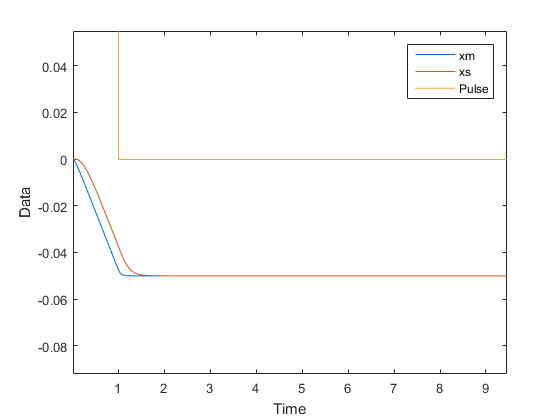
\includegraphics[width=0.5\linewidth]{images/Predet2.PNG}
		\caption{Modelo con valores predeterminados dados para el Fuerza-Posición.}
		\label{Predet Values F-P}
	\end{figure}
	\FloatBarrier
	
	Modificándose el valor del rozamiento del maestro, $B_m$, se obtiene los resultados de la Figura \ref{Master_Friction-FP}. Y se observa que cuanto mayor es $B_m$ menor es la amplitud de respuesta del maestro y del esclavo ante un mismo pulso de fuerza. Estas respuestas son lógicas, ya que cuando el medio o internamente el propio robot posee fricciones ante una misma fuerza el maestro se desplaza menos, al haber una fuerza que se le contrapone dependiente de la velocidad a la que se mueva el maestro.\\
	
	\begin{figure}[h!]
		\centering
		\begin{subfigure}[t]{.5\textwidth}
			\centering
			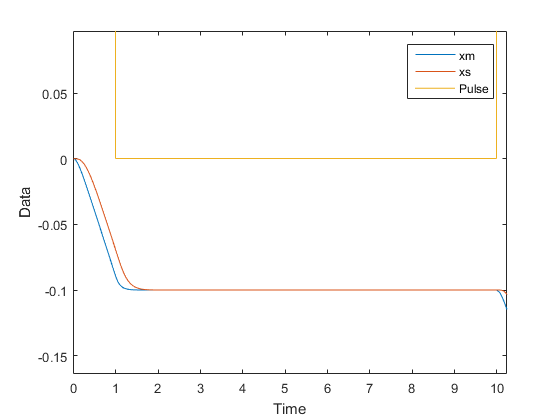
\includegraphics[width=1\linewidth]{images/Bm10-FP.PNG}
			\caption{Con $B_m = 10$}
			\label{Bm10-FP}
		\end{subfigure}%
		\begin{subfigure}[t]{.5\textwidth}
			\centering
			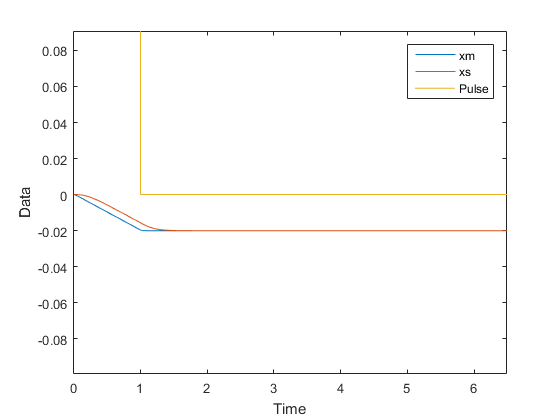
\includegraphics[width=1\linewidth]{images/Bm50-FP.PNG}
			\caption{Con $B_m = 50$}
			\label{Bm50-FP}
		\end{subfigure}
		\begin{subfigure}[t]{.5\textwidth}
			\centering
			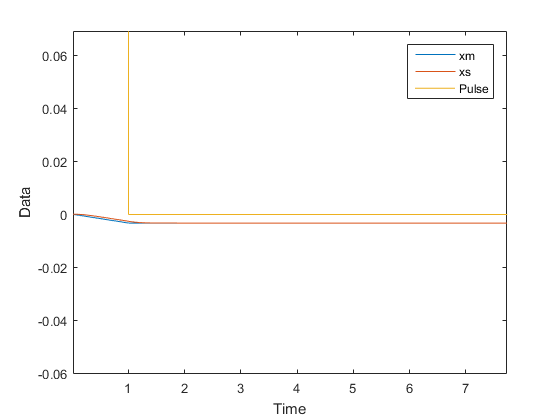
\includegraphics[width=1\linewidth]{images/Bm300-FP.PNG}
			\caption{Con $B_m = 300$}
			\label{Bm300-FP}
		\end{subfigure}
		\caption{Respuestas con distintos coeficientes de fricción en el Maestro}
		\label{Master_Friction-FP}
	\end{figure}
	\FloatBarrier
	
	Manteniendo $B_m = 20$, modificamos el coeficiente $B_s$ de fricción del esclavo, obteniendo las respuestas de las Figuras \ref{Slave_Friction-FP}. Se observa que las amplitudes de respuestas son parecidas, pero varía mucho las formas de la respuesta del sistema esclavo, esto es entendible ya que ante un mismo movimiento del maestro el esclavo actúa cada vez con menor movimiento, la fricción se contrapone al movimiento. En la Figura \ref{Bs10-FP} incluso se observa que el esclavo se desplaza más de lo debido creando una pequeña oscilación, pero como el bucle de realimentación al maestro tiene valor nulo, este no muestra una sobreoscilación. Al crecer la $B_s$ las diferencias en ambas respuestas, Maestro y Esclavo, tendrán cada vez mayores discrepancias.\\
	
	\begin{figure}[h!]
		\centering
		\begin{subfigure}[t]{.5\textwidth}
			\centering
			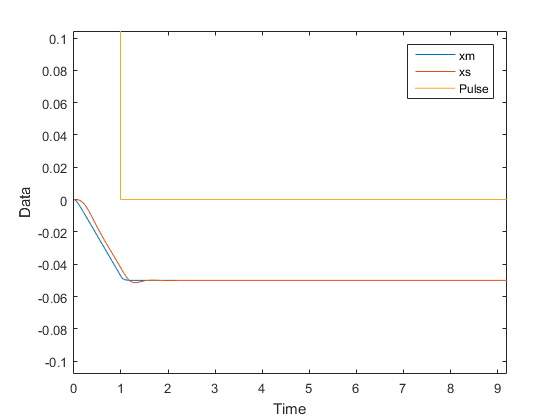
\includegraphics[width=1\linewidth]{images/Bs10-FP.PNG}
			\caption{Con $B_s = 10$}
			\label{Bs10-FP}
		\end{subfigure}%
		\begin{subfigure}[t]{.5\textwidth}
			\centering
			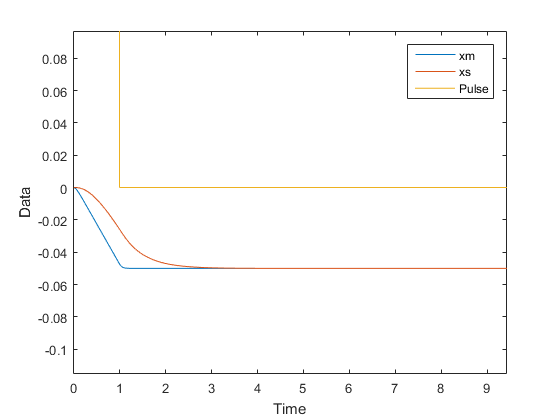
\includegraphics[width=1\linewidth]{images/Bs50-FP.PNG}
			\caption{Con $B_s = 50$}
			\label{Bs30-FP}
		\end{subfigure}
		\begin{subfigure}[t]{.5\textwidth}
			\centering
			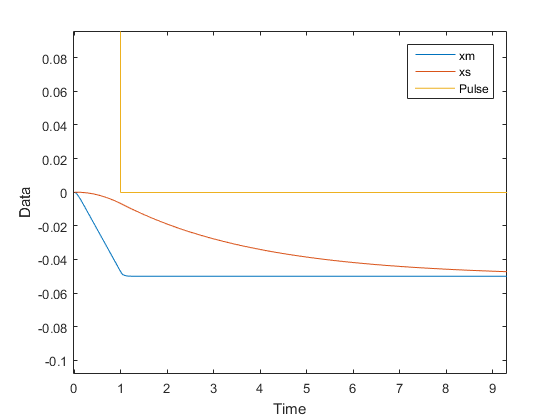
\includegraphics[width=1\linewidth]{images/Bs300-FP.PNG}
			\caption{Con $B_s = 300-FP$}
			\label{Bs300-FP}
		\end{subfigure}
		\caption{Respuestas con distintos coeficientes de fricción en el Esclavo}
		\label{Slave_Friction-FP}
	\end{figure}
	\FloatBarrier
	
	Todos estos casos en los que se han modificado los coeficientes de fricción se han realizado con un $K_e = 0$, por tanto el movimiento es libre, además si se mira el esquema Fuerza-Posición, Figura \ref{Force-Position Control Scheme}, se ve que al tener $K_e$ un valor nulo también la fuerza realimentada al maestro será nula, por lo que el sistema pierde parte de su bilateralidad. Por tanto habrá que estudiar casos con $K_e > 0$, es decir el caso de estar en un entorno elástico y con fricción y/o viscosidad de $B_m = 20$ y $B_s = 20$. Además hay que ajustar el coeficiente $Kf$ a $0.5$ para conseguir que el sistema no muestre fuertes inestabilidades ante pequeñas variaciones de $K_e$. Se obtendrán las respuestas de la Figura \ref{Slave_Stifnes-FP}. Al aumentar el coeficiente de elasticidad con el entorno la respuesta de esclavo actuará con idéntica rapidez, pero irá creciendo en error de posición con respecto a la posición del maestro al dejar de aplicar la fuerza del operario. Este fenómeno se entiende como que cada vez cuesta más mover el esclavo debido a la existencia de ese \textquotedblleft muelle \textquotedblright. Se ve que entorno a $K_e = 10$ la respuesta final del Maestro no será tan constante, sino que aunque no haya una fuerza que se esté aplicando la realimentación de la fuerza producida por el entorno causará cada vez un mayor desplazamiento en la posición del maestro. Al aumentar mucho la $K_e$ cualquier mínima variación de la posición del esclavo producirá grandes fuerzas a la entrada del maestro.
	
	\begin{figure}[h!]
		\centering
		\begin{subfigure}[t]{.5\textwidth}
			\centering
			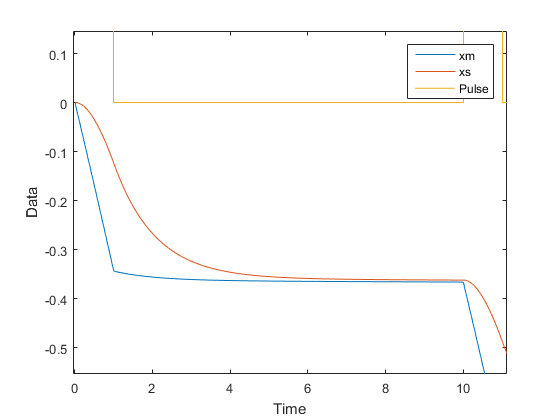
\includegraphics[width=1\linewidth]{images/Ke1.PNG}
			\caption{Con $K_e = 1$}
			\label{Ke1-FP}
		\end{subfigure}%
		\begin{subfigure}[t]{.5\textwidth}
			\centering
			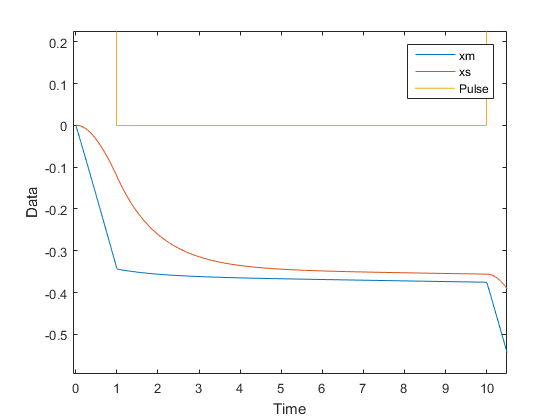
\includegraphics[width=1\linewidth]{images/Ke5.PNG}
			\caption{Con $K_e = 5$}
			\label{Ke5-FP}
		\end{subfigure}
		\begin{subfigure}[t]{.5\textwidth}
			\centering
			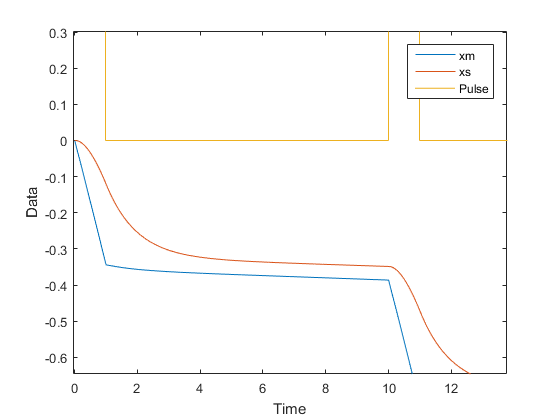
\includegraphics[width=1\linewidth]{images/Ke10.PNG}
			\caption{Con $K_e = 10$}
			\label{Ke10-FP}
		\end{subfigure}
		\caption{Respuestas con distintos coeficientes de elasticidad, $K_e$, en el sistema esclavo}
		\label{Slave_Stifnes-FP}
	\end{figure}
	\FloatBarrier
	
	\bibliographystyle{acm} % estilo de la bibliografía.
	\bibliography{yyyy} 
	
	\begin{thebibliography}{X}
		
		\bibitem{Bilateral} \textsc{Manuel Ferre, Jordi Barrio, Claudio Melchiorri, Juan M. Bogado, Pedro L. Castedo} y \textsc{Juan M. Ibarra}. \textit{Experimental Results on Bilateral Control Using an Industrial Telemanipulator}. En \textit{Advances in Telerrobotics}, páginas 177-190.
		
	
		
	\end{thebibliography}
	
\end{document}